\documentclass[a4paper, twoside, openany, parskip=half, 10pt]{article}
\usepackage[a4paper, top=1cm, bottom=1cm, inner=1cm, outer=1cm, marginparsep=.1cm, headsep=16pt, landscape]{geometry}
\setlength{\marginparwidth}{1cm}

\usepackage{siddur}
\usepackage{background}

\backgroundsetup{
  scale=1,       % Scale the image if needed; 1 means the image is at its original size
  color=black,  % Color of the contents of the page, not the background
  opacity=0.3,  % Opacity of the background; 1 is fully opaque, 0 is fully transparent
  angle=0,      % Rotation angle of the background (in degrees)
  position=current page.south, % Position; you can also use 'current page.center' etc.
  vshift=10.5cm,  % Vertical shift for manual positioning
  hshift=0cm,   % Horizontal shift for manual positioning
  contents={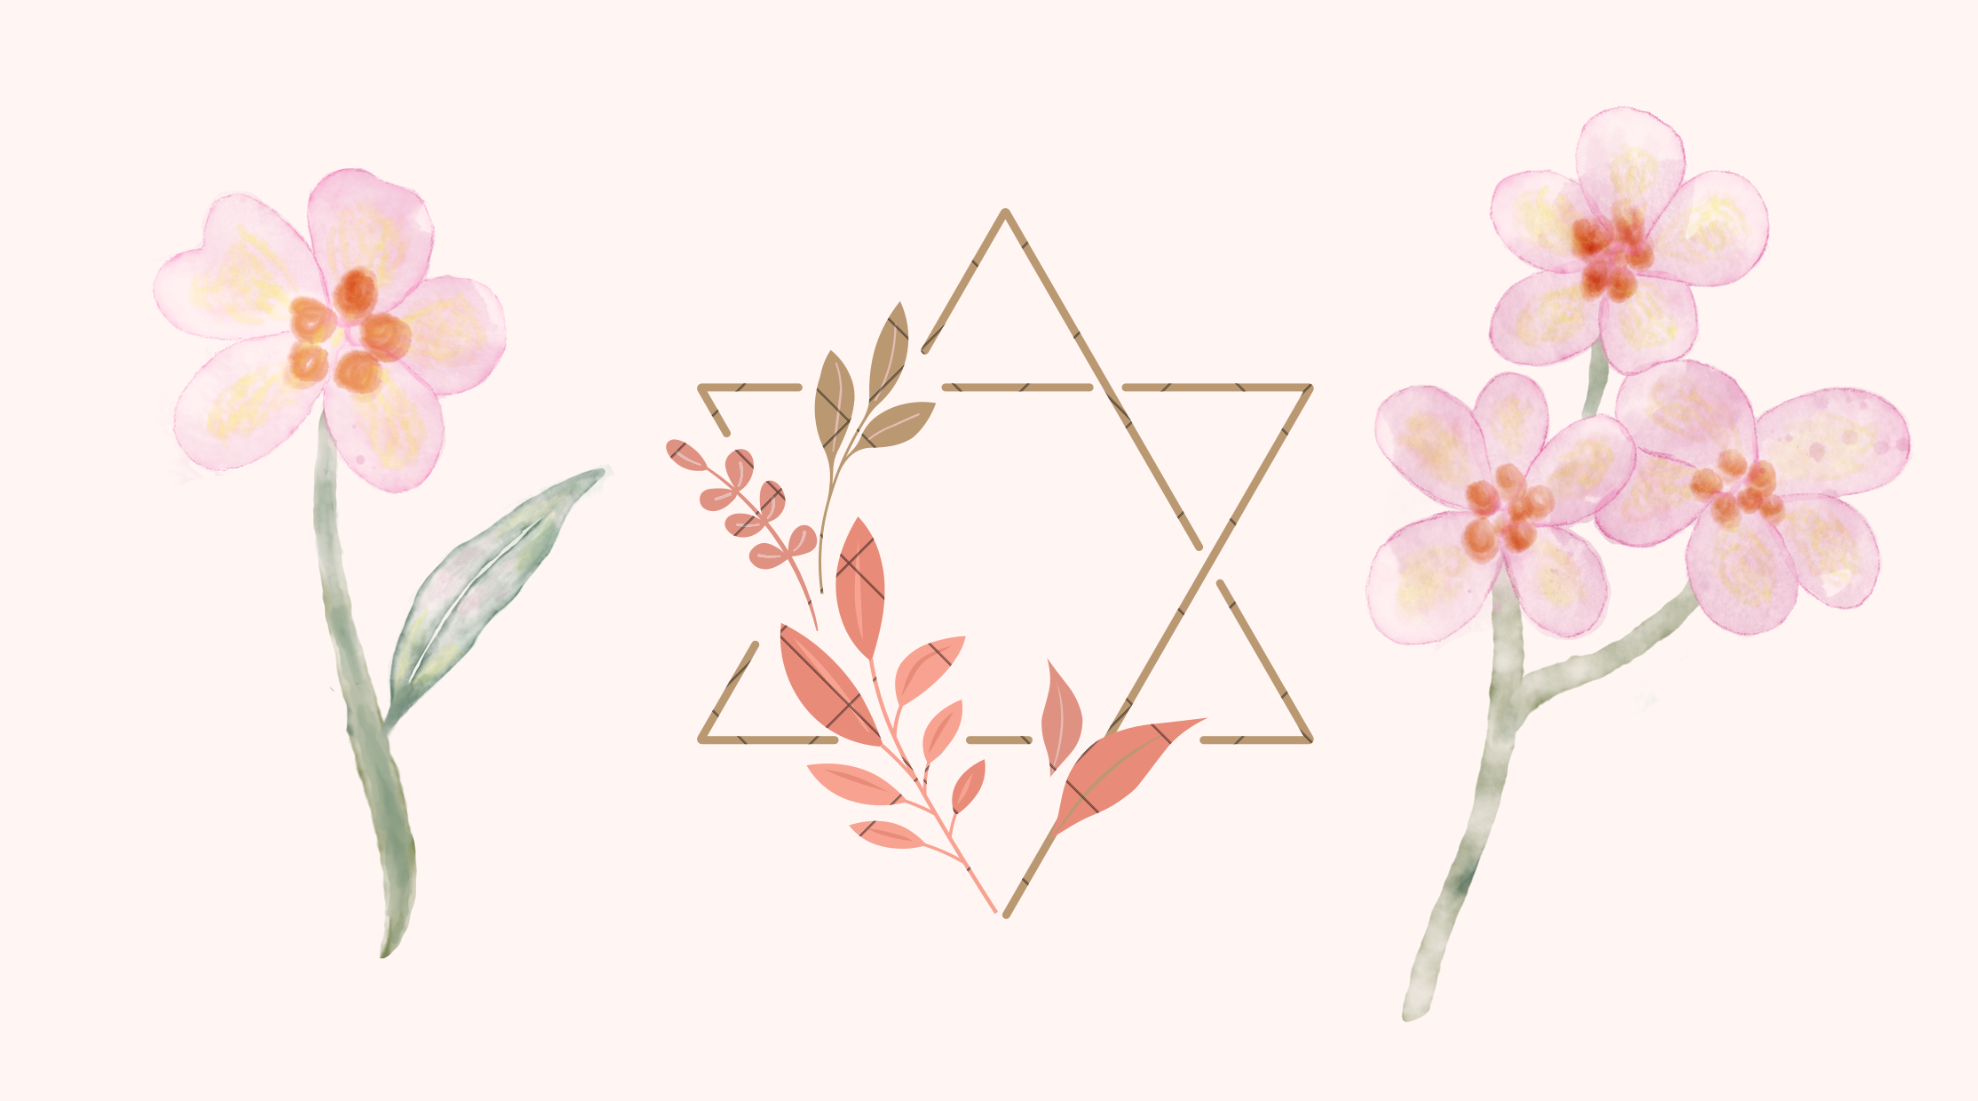
\includegraphics[width=\paperwidth,height=\paperheight]{bg.png}}  % Path to the image file
}


\usepackage{xcolor}

\definecolor{gold}{HTML}{896132}
\definecolor{darkGrey}{HTML}{545454}
\setlength{\columnsep}{15pt}

\begin{document}

%remove page numbering imported from siddur.sty
\pagenumbering{gobble}

I don't know why the first page's background doesn't get opacity.

\nextpage



\begin{multicols}{3}

\begin{Large}
\textcolor{darkGrey}{
בת המצווה של
}
\end{Large}

\begin{Huge}
\textcolor{gold}{
דבורה רות וולף
}
\end{Huge}

\begin{large}
\textcolor{darkGrey}{
שבת פרשת חיי שרה\\
כ״ז בחשון תשפ״ד\\
}

\end{large}





%\section{\adforn{47} ברכת המזון \adforn{19}}




\firstword{שִׁ֗יר הַֽמַּֽ֫עֲל֥וֹת}
בְּשׁ֣וּב יְ֖יָ אֶת־שִׁיבַ֣ת צִיּ֑וֹן הָ֝יִ֗ינוּ כְּחֹלְֿמִֽים׃ 
 אָ֤ז יִמָּלֵ֢א שְׂחֹ֡ק פִּינוּ֘ וּלְשׁוֹנֵ֢נוּ רִ֫נָּ֥ה אָ֭ז יֹֽאמְֿר֣וּ בַגּוֹיִ֑ם הִגְדִּ֥יל יְ֜יָ֗ לַֽעֲשׂ֥וֹת עִם־אֵֽלֶּה׃ 
 הִגְדִּ֥יל יְ֖יָ לַֽעֲשׂ֣וֹת עִמָּ֑נוּ הָ֜יִ֗ינוּ שְׂמֵחִֽים׃ 
 שׁוּבָ֣ה יְ֖יָ אֶת־שְׁבִותֵ֑נוּ כַּֽאֲפִיקִ֥ים בַּנֶּֽגֶב׃ 
 הַזֹּֽרְֿעִ֥ים בְּדִמְעָ֗ה בְּרִנָּ֥ה יִקְצֹֽרוּ׃ 
 הָ֘ל֤וֹךְ יֵלֵ֨ךְ וּבָכֹה֘ נֹשֵׂ֢א מֶֽשֶׁךְ־הַ֫זָּ֥רַע בֹּֽא־יָבֹ֥א בְרִנָּ֗ה נֹשֵׂ֥א אֲלֻמֹּתָֽיו׃ \\


\instruction{המזמן:}
רַבּוֹתַי נְבָרֵךְ! \hfill \break
\instruction{כולם:}
 יְהִ֤י שֵׁ֣ם יְיָ֣ מְבֹרָ֑ךְ מֵֽ֝עַתָּ֗ה וְעַד־עוֹלָֽם׃\hfill \break
\instruction{המזמן:}
בִּרְשׁוּת ... נְבָרֵךְ (\instruction{בעשרה} אֱלֹהֵֽינוּ) שֶׁאָכַלְנוּ מִשֶּׁלּוֹ:\hfill \break
\instruction{כולם:}
בָּרוּךְ (\instruction{בעשרה:} אֱלֹהֵֽינוּ) שֶׁאָכַֽלְנוּ מִשֶּׁלּוֹ וּבְטוּבוֹ חָיִֽינוּ:\hfill \break
%(\instruction{מי שלא אכל:}
%בָּרוּךְ וּמְבֹרָךְ שְׁמוֹ תָּמִיד לְעוֹלָם וָעֶד:)\hfill \break
\instruction{המזמן:}
בָּרוּךְ (\instruction{בעשרה:} אֱלֹהֵֽינוּ) שֶׁאָכַֽלְנוּ מִשֶּׁלּוֹ וּבְטוּבוֹ חָיִֽינוּ:\hfill \break
\instruction{כולם:}
 בָּרוּךְ הוּא וּבָרוּךְ שְׁמוֹ:\hfill \break


\firstword{בָּרוּךְ}
אַתָּה יְיָ אֱלֹהֵֽינוּ מֶֽלֶךְ הָעוֹלָם הַזָּן אֶת הָעוֹלָם כֻּלּוֹ בְּטוּבוֹ בְּחֵן בְּחֶֽסֶד וּבְרַחֲמִים הוּא נֹתֵ֣ן \source{תהלים קלו}לֶ֭חֶם לְכָל־בָּשָׂ֑ר כִּ֖י לְעוֹלָ֣ם חַסְדּֽוֹ: וּבְטוּבוֹ הַגָּדוֹל תָּמִיד לֹא חָסַר לָֽנוּ וְאַל יֶחְסַר לָֽנוּ מָזוֹן לְעוֹלָם וָעֶד: בַּעֲבוּר שְׁמוֹ הַגָּדוֹל כִּי הוּא זָן וּמְפַרְנֵס לַכֹּל וּמֵטִיב לַכֹּל וּמֵכִין מָזוֹן לְכָל בְּרִיּוֹתָיו אֲשֶׁר בָּרָא: בָּרוּךְ אַתָּה יְיָ הַזָּן אֶת הַכֹּל:\\

\firstword{נוֹדֶה}
	לְּךָ יְיָ אֱלֹהֵֽינוּ עַל שֶׁהִנְחַֽלְתָּ לַאֲבוֹתֵֽינוּ אֶֽרֶץ חֶמְדָה טוֹבָה וּרְחָבָה: וְעַל שֶׁהוֹצֵאתָֽנוּ יְיָ אֱלֹהֵֽינוּ מֵאֶֽרֶץ מִצְרַֽיִם וּפְדִיתָֽנוּ מִבֵּית עֲבָדִים וְעַל בְּרִיתְֿךָ שֶׁחָתַֽמְתָּ בִּבְשָׂרֵֽנוּ וְעַל תּוֹרָתְֿךָ שֶׁלִּמַּדְתָּֽנוּ וְעַל חֻקֶּֽיךָ שֶׁהוֹדַעְתָּֽנוּ וְעַל חַיִּים חֵן וָחֶֽסֶד שֶׁחוֹנַנְתָּֽנוּ וְעַל אֲכִילַת מָזוֹן שָׁאַתָּה זָן וּמְפַרְנֵס אוֹתָֽנוּ תָּמִיד בְּכָל יוֹם וּבְכָל עֵת וּבְכָל שָׁעָה:

\begin{sometimes}
\firstword{עַל הַנִּסִּים}
 וְעַל הַפֻּרְקָן וְעַל הַגְּֿבוּרוֹת וְעַל הַתְּֿשׁוּעוֹת וְעַל הַמִּלְחָמוֹת שֶׁעָשִֽׂיתָ לַאֲבוֹתֵֽינוּ בַּיָּמִים הָהֵם בַּזְּֿמַן זֶּה:
 
\instruction{בחנוכה:}
בִּימֵי מַתִּתְיָֽהוּ בֶּן יוֹחָנָן כֹּהֵן גָּדוֹל חַשְׁמֹנַי וּבָנָיו כְּשֶׁעָמְֿדָה מַלְכוּת יָוָן הָרְֿשָׁעָה עַל עַמְּֿךָ יִשְׂרָאֵל לְהַשְׁכִּיחָם תּוֹרָתֶֽךָ וּלְהַעֲבִירָם מֵחֻקֵּי רְצוֹנֶֽךָ: וְאַתָּה בְּרַחֲמֶֽיךָ הָרַבִּים עָמַֽדְתָּ לָהֶם בְּעֵת צָרָתָם רַֽבְתָּ אֶת רִיבָם דַּֽנְתָּ אֶת דִּינָם נָקַֽמְתָּ אֶת נִקְמָתָם: מָסַֽרְתָּ גִּבּוֹרִים בְּיַד חַלָּשִׁים וְרַבִּים בְּיַד מְעַטִּים וּטְמֵאִים בְּיַד טְהוֹרִים וּרְשָׁעִים בְּיַד צַדִּיקִים וְזֵדִים בְּיַד עוֹסְֿקֵי תוֹרָתֶֽךָ: וּלְךָ עָשִֽׂיתָ שֵׁם גָּדוֹל וְקָדוֹשׁ בְּעוֹלָמֶֽךָ וּלְעַמְּֿךָ יִשְׂרָאֵל עָשִֽׂיתָ תְּשׁוּעָה גְדוֹלָה וּפֻרְקָן כְּהַיּוֹם הַזֶּה: וְאַֽחַר כַּךְ בָּֽאוּ בָנֶֽיךָ לִדְבִיר בֵּיתֶֽךָ וּפִנּוּ אֶת הֵיכָלֶֽךָ וְטִהֲרוּ אֶת מִקְדָּשֶֽׁךָ וְהִדְלִֽיקוּ נֵרוֹת בְּחַצְרוֹת קָדְּֿשֶֽׁךָ וְקָבְֿעוּ שְׁמוֹנַת יְמֵי חֲנֻכָּה אֵֽלּוּ לְהוֹדוֹת לְהַלֵּל לְשִׁמְךָ הַגָּדוֹל: 

\instruction{בפורים:}
בִּימֵי מָרְדֳּכַי וְִאֶסְתֵּר בְּשׁוּשַׁן הַבִּירָה כְּשֶׁעָמַד עֲלֵיהֶם הָמָן הָרָשָׁע בִּקֵּשׁ
 לְהַשְׁמִ֡יד לַֽהֲרֹ֣ג וּלְאַבֵּ֣ד אֶת־כָּל־הַ֠יְּֿהוּדִים מִנַּ֨עַר וְעַד־זָקֵ֨ן טַ֤ף וְנָשִׁים֙ בְּי֣וֹם אֶחָ֔ד בִּשְׁלוֹשָׁ֥ה עָשָׂ֛ר לְחֹ֥דֶשׁ שְׁנֵים־עָשָׂ֖ר הוּא־חֹ֣דֶשׁ אֲדָ֑ר וּשְׁלָלָ֖ם לָבֽוֹז׃ וְאַתָּה בְּרַחֲמֶֽיךָ הָרַבִּים הֵפַֽרְתָּ אֶת עֲצָתוֹ וְקִלְקַלְתָּ אֶת מַחֲשַׁבְתּוֹ וַהֲשֵׁבֽוֹתָ גְּמוּלוֹ בְּרֹאשׁוֹ וְתָלוּ אוֹתוֹ וְאֶת בָּנָיו עַל הָעֵץ:

\end{sometimes}

\firstword{וְעַל הַכֹּל}
 יְיָ אֱלֹהֵֽינוּ אָֽנוּ מוֹדִים לָךְ וּמְבָרֲכִים אוֹתָךְ יִתְבָּרַךְ שִׁמְךָ בְּפִי כָל חַי תָּמִיד לְעוֹלָם וָעֶד: כַּכָּתוּב: \source{דברים ח}וְאָֽכַלְתָּ֖ וְשָׂבָ֑עְתָּ וּבֵֽרַכְתָּ֙ אֶת־יְיָ֣ אֱלֹהֶ֔יךָ עַל־הָאָ֥רֶץ הַטֹּבָ֖ה אֲשֶׁ֥ר נָֽתַן־לָֽךְ׃ בָּרוּךְ אַתָּה יְיָ עַל הָאָֽרֶץ וְעַל הַמָּזוֹן:\\

\firstword{רַחֵם}
 יְיָ אֱלֹהֵֽינוּ עָלֵֽינוּ וְעַל יִשְׂרָאֵל עַמֶּךָ וְעַל יְרוּשָׁלַֽםִ עִירֶֽךָ וְעַל צִיּוֹן מִשְׁכַּן כְּבוֹדֶֽךָ וְעַל מַלְכוּת בֵּית דָּוִד מְשִׁיחֶֽךָ וְעַל הַבַּֽיִת הַגָּדוֹל וְהַקָּדוֹשׁ שֶׁנִּקְרָא שִׁמְךָ עָלָיו: אֱלֹהֵֽינוּ אָבִֽינוּ רְעֵֽנוּ זוּנֵֽנוּ פַרְנְֿסֵֽנוּ וְכַלְכְּֿלֵֽנוּ וְהַרְוִיחֵֽנוּ וְהַרְוַח לָֽנוּ יְיָ אֱלֹהֵֽינוּ מְהֵרָה מִכָּל צָרוֹתֵֽינוּ: וְנָא אַל תַּצְרִיכֵֽנוּ יְיָ אֱלֹהֵֽינוּ לֹא לִידֵי מַתְּֿנַת בָּשָׂר וָדָם וְלֹא לִידֵי הַלְוָאָתָם אֶלָּא לְיָדְֿךָ הַמְּֿלֵאָה הַפְּֿתוּחָה הַקְּֿדוֹשָׁה וְהָרְֿחָבָה שֶׁלֹּא נֵבוֹשׁ וְלֹא נִכָּלֵם לְעוֹלָם וָעֶד:

\begin{sometimes}

\shabbos 
רְצֵה וְהַחֲלִיצֵֽנוּ יְיָ אֱלֹהֵֽינוּ בְּמִצְוֹתֶֽיךָ וּבְמִצְוַת יוֹם הַשְּֿׁבִיעִי הַשַּׁבָּת הַגָּדוֹל וְהַקָּדוֹשׁ הַזֶּה כִּי יוֹם זֶה גָּדוֹל וְקָדוֹשׁ הוּא לְפָנֶֽיךָ לִשְׁבָּת בּוֹ וְלָנֽוּחַ בּוֹ בְּאַהֲבָה כְּמִצְוַת רְצוֹנֶךָ: בִּרְצוֹנְֿךָ הָנִֽיחַ לָֽנוּ יְיָ אֱלֹהֵֽינוּ שֶׁלֹא תְהֵי צָרָה וְיָגוֹן וַאֲנָחָה בְּיוֹם מְנוּחָתֵֽנוּ וְהַרְאֵֽנוּ יְיָ אֱלֹהֵֽינוּ בְּנֶחָמוֹת צִיּוֹן עִירֶֽךָ וּבְֿבִנְיַן יְרוּשָׁלַֽםִ עִיר קָדְשֶֽׁךָ כִּי אַתָּה הוּא בַּֽעַל הַיְשׁוּעוֹת וּבַֽעַל הַנֶּחָמוֹת: 

\sepline %These are really two "sometimes's". Sepline to separate them

%\vspace{-.25\baselineskip}
\instruction{בר"ח ומועדים:}
אֱלֹהֵֽינוּ וֵאלֹהֵי אֲבוֹתֵֽינוּ יַעֲלֶה וְיָבֹא וְיַגִּיעַ וְיֵרָאֶה וְיֵרָצֶה וְיִשָּׁמַע וְיִפָּקֵד וְיִזָּכֵר זִכְרוֹנֵֽנוּ וּפִקְדּוֹנֵֽנוּ וְזִכְרוֹן אֲבוֹתֵֽינוּ וְזִכְרוֹן מָשִׁיחַ בֶּן דָּוִד עַבְדֶּֽךָ וְזִכְרוֹן יְרוּשָׁלַֽםִ עִיר קָדְשֶֽׁךָ וְזִכְרוֹן כָּל עַמְּֿךָ בֵּית יִשְׂרָאֵל לְפָנֶיךָ לִפְלֵיטָה וּלְטוֹבָה וּלְחֵן וּלְחֶֽסֶד וּלְרַחֲמִים וּלְחַיִּים וּלְשָׁלוֹם בְּיוֹם\\ 
\begin{tabular}{c|c|c}
 רֹאשׁ הַחֹֽדֶשׁ & חַג הַמַּצוֹת & חַג הַשָּׁבֻעוֹת\\ \hline
 \end{tabular}\\
\begin{tabular}{c|c|c}
 הַזִּכָּרוֹן & חַג הַסֻּכּוֹת & שְׁמִינִי חַג הָעֲצֶֽרֶת
\end{tabular}\\
הַזֶּה זָכְרֵֽנּוּ יְיָ אֱלֹהֵֽינוּ בּוֹ לְטוֹבָה וּפָקְדֵֽנוּ בוֹ לִבְרָכָה וְהוֹשִׁיעֵֽנוּ בוֹ לְחַיִּים וּבִדְבַר יְשׁוּעָה וְרַחֲמִים חוּס וְחָנֵּנוּ וְרַחֵם עָלֵֽינוּ וְהוֹשִׁיעֵֽנוּ כִּי אֵלֶֽיךָ עֵינֵֽינוּ כִּי אֵל מֶֽלֶךְ חַנּוּן וְרַחוּם אַֽתָּה:

\end{sometimes}

\firstword{וּבְנֵה}
 יְרוּשָׁלַֽםִ עִיר הַקֹּֽדֶשׁ בִּמְהֵרָה בְּיָמֵֽינוּ: בָּרוּךְ אַתָּה יְיָ בֹּֽנֶה בְרַחֲמָיו יְרוּשָׁלָֽםִ אָמֵן:\\

\firstword{בָּרוּךְ}
 אַתָּה יְיָ אֱלֹהֵֽינוּ מֶֽלֶךְ הָעוֹלָם הָאֵל אָבִֽינוּ מַלְכֵּֽנוּ אַדִּירֵֽנוּ בּוֹרְֿאֵֽנוּ גֹאֲלֵֽנוּ יוֹצְֿרֵֽנוּ קְדוֹשֵֽׁנוּ קְדוֹשׁ יַעֲקֹב רוֹעֵֽנוּ רוֹעֵה יִשְׂרָאֵל הַמֶּֽלֶךְ הַטּוֹב וְהַמֵּטִיב לַכֹּל שֶׁבְּכָל יוֹם וָיוֹם הוּא הֵטִיב הוּא מֵטִיב הוּא יֵיטִיב לָֽנוּ: הוּא גְמָלָֽנוּ הוּא גוֹמְֿלֵנוּ הוּא יִגְמְֿלֵנוּ לָעַד לְחֵן לְחֶֽסֶד וּלְרַחֲמִים וּלְרֶֽוַח הַצָּלָה וְהַצְלָחָה בְּרָכָה וִישׁוּעָה נֶחָמָה פַּרְנָסָה וְכַלְכָּלָה וְרַחֲמִים וְחַיִּים וְשָׁלוֹם וְכָל טוֹב וּמִכָּל טוֹב אַל יְחַסְּֿרֵֽנוּ:\\

\columnbreak

\begin{sometimes}

\instruction{אם שכח בשבת לומר 'רצה':}\\
בָּרוּךְ אַתָּה יְיָ אֱלֹהֵֽינוּ מֶֽלֶךְ הָעוֹלָם אֲשֶׁר נָתַן שַׁבָּתוֹת לִמְנוּחָה לְעַמּוֹ יִשְׂרָאֵל בְּאַהֲבָה 
לְאוֹת וְלִבְרִית: בָּרוּךְ אַתָּה יְיָ מְקַדֵּשׁ הַשַּׁבָּת:


\instruction{אם שכח לומר 'יעלה ויבא' בראש חדש:}\\
בָּרוּךְ אַתָּה יְיָ אֱלֹהֵֽינוּ מֶֽלֶךְ הָעוֹלָם 
אֲשֶׁר נָתַן רָאשֵׁי חֳדָשִׁים לְעַמּוֹ יִשְׂרָאֵל לְזִכָּרוֹן:

\instruction{אם שכח שבת ראש חודש 'רצה' ו'יעלה ויבא':}\\
בָּרוּךְ אַתָּה יְיָ אֱלֹהֵֽינוּ מֶֽלֶךְ הָעוֹלָם 
אֲשֶׁר נָתַן שַׁבָּתוֹת לִמְנוּחָה לְעַמּוֹ יִשְׂרָאֵל בְּאַהֲבָה לְאוֹת וְלִבְרִית וְרָאשֵׁי חֳדָשִׁים לְזִכָּרוֹן: 
בָּרוּךְ אַתָּה יְיָ מְקַדֵּשׁ הַשַּׁבָּת וְיִשְׂרָאֵל וְרָאשֵׁי חֳדָשִׁים:

\instruction{אם שכח 'יעלה ויבא' ביום טוב:}\\
בָּרוּךְ אַתָּה יְיָ אֱלֹהֵֽינוּ מֶֽלֶךְ הָעוֹלָם 
אֲשֶׁר נָתַן יָמִים טוֹבִים לְעַמּוֹ יִשְׂרָאֵל 
לְשָׂשׂוֹן וּלְשִׂמְחָה אֶת־יוֹם חַג
הַמַּצּוֹת \textbackslash הַשָּׁבֻעוֹת \textbackslash הַסֻּכּוֹת \textbackslash  שְׁמִינִי חַג הָעֲצֶֽרֶת הַזֶּה:
 הַזֶּה: 
בָּרוּךְ אַתָּה יְיָ מְקַדֵּשׁ יִשְׂרָאֵל וְהַזְּמַנִּים:

\instruction{אם שכח שבת יום טוב 'רצה' ו'יעלה ויבא':}\\
בָּרוּךְ אַתָּה יְיָ אֱלֹהֵֽינוּ מֶֽלֶךְ הָעוֹלָם אֲשֶׁר נָתַן שַׁבָּתוֹת לִמְנוּחָה לְעַמּוֹ יִשְׂרָאֵל בְּאַהֲבָה לְאוֹת וְלִבְרִית 
וְיָמִים טוֹבִים לְשָׂשׂוֹן וּלְשִׂמְחָה אֶת־יוֹם חַג הַמַּצּוֹת \textbackslash הַשָּׁבֻעוֹת \textbackslash הַסֻּכּוֹת \textbackslash  שְׁמִינִי חַג הָעֲצֶֽרֶת הַזֶּה: הַזֶּה: 
בָּרוּךְ אַתָּה יְיָ מְקַדֵּשׁ הַשַּׁבָּת וְיִשְׂרָאֵל וְהַזְּמַנִּים:

\end{sometimes}


\firstword{בָּרוּךְ}
 אַתָּה יְיָ אֱלֹהֵֽינוּ מֶֽלֶךְ הָעוֹלָם הָאֵל אָבִֽינוּ מַלְכֵּֽנוּ אַדִּירֵֽנוּ בּוֹרְֿאֵֽנוּ גֹאֲלֵֽנוּ יוֹצְֿרֵֽנוּ קְדוֹשֵֽׁנוּ קְדוֹשׁ יַעֲקֹב רוֹעֵֽנוּ רוֹעֵה יִשְׂרָאֵל הַמֶּֽלֶךְ הַטּוֹב וְהַמֵּטִיב לַכֹּל שֶׁבְּכָל יוֹם וָיוֹם הוּא הֵטִיב הוּא מֵטִיב הוּא יֵיטִיב לָֽנוּ: הוּא גְמָלָֽנוּ הוּא גוֹמְֿלֵנוּ הוּא יִגְמְֿלֵנוּ לָעַד לְחֵן לְחֶֽסֶד וּלְרַחֲמִים וּלְרֶֽוַח הַצָּלָה וְהַצְלָחָה בְּרָכָה וִישׁוּעָה נֶחָמָה פַּרְנָסָה וְכַלְכָּלָה וְרַחֲמִים וְחַיִּים וְשָׁלוֹם וְכָל טוֹב וּמִכָּל טוֹב אַל יְחַסְּֿרֵֽנוּ:\\

%\instruction{יש שמסיימים כאן בשבת.}

\firstword{הָרַחֲמָן}
 הוּא יִמְלֹךְ עָלֵֽינוּ לְעוֹלָם וָעֶד: 
	\firstword{הָרַחֲמָן}
	 הוּא יִתְבָּרַךְ בַּשָּׁמַֽיִם וּבָאָֽרֶץ: 
	\firstword{הָרַחֲמָן}
	 הוּא יִשְׁתַּבַּח לְדוֹר דּוֹרִים וְיִתְפָּֽאַר בָּֽנוּ לָנֵֽצַח נְצָחִים 
		 וְיִתְהַדַּר בָּֽנוּ לָעַד וּלְעוֹלְֿמֵי עוֹלָמִים: 
	\firstword{הָרַחֲמָן}
	 הוּא יְפַרְנְֿסֵֽנוּ בְּכָבוֹד: 
	\firstword{הָרַחֲמָן}
	 הוּא יִשְׁבּוֹר עֹל גּוֹיִם מֵעַל צַוָּארֵֽנוּ וְהוּא יוֹלִיכֵֽנוּ קוֹמֲמִיּוּת לְאַרְצֵֽנוּ: 
	\firstword{הָרַחֲמָן}
	 הוּא יִשְׁלַח בְּרָכָה מְרֻבָּה בְּבַֽיִת זֶה וְעַל שֻׁלְחָן זֶה שֶׁאָכַֽלְנוּ עָלָיו: 
\firstword{הָרַחֲמָן}
 הוּא יִשְׁלַח לָֽנוּ אֶת אֵלִיָּֽה הַנָּבִיא זָכוּר לַטּוֹב וִיבַשֵּׂר לָנוּ בְּשׂוֹרוֹת טוֹבוֹת יְשׁוּעוֹת וְנֶחָמוֹת:\\


\begin{footnotesize}
\instruction{אורחים אומרים:}\\
יְהִי רָצוֹן שֶׁלֹא יֵבוֹשׁ בַּעַל הַבַּיִת בָּעוֹלָם הַזֶּה וְלֹא יִכָּלֵם לָעוֹלָם הַבָּא וְיִצְלַח מְאֹד בְּכָל נְכָסָיו וְיִהְיוּ נְכָסָיו מֻצְלָחִים וּקְרוֹבִים לָעִיר וְאַל יִשְׁלוֹט שָׂטָן לֹא בְּמַעֲשֵׂי יָדָיו וְלֹא בְּמַעֲשֵׂי יָדֵינוּ וְאַל יִזְדַקֵּר לֹא לְפָנָיו וְלֹא לְפָנֵינוּ שׁוּם דְבַר הִרְהוּר חֵטְא וַעֲבֵרָה וְעָוֹן מֵעַתָּה וְעַד עוֹלָם:\\

\end{footnotesize}
 
\firstword{הָרַחֲמָן}
 הוּא יְבָרֵךְ אֶת [אָבִי מוֹרִי] בַּעַל הַבַּֽיִת הַזֶּה וְאֶת [אִמִּי מוֹרָתִי] בַּעֲלַת הַבַּֽיִת הַזֶּה: אוֹתָם וְאֶת בֵּיתָם וְאֶת זַרְעָם וְאֶת כָּל אַשֶׁר לָהֶם, אוֹתָנוּ וְאֶת כָּל אַשֶׁר לָֽנוּ כְּמוֹ שֶׁנִּתְבָּרֲכוּ אֲבוֹתֵֽינוּ אַבְרָהָם יִצְחָק וְיַעֲקֹב בַּכֹּל מִכֹּל כֹּל כֵּן יְבָרֵךְ אוֹתָֽנוּ כֻּלָּנוּ יַֽחַד בִּבְרָכָה שְׁלֵמָה וְנֹאמַר אָמֵן:\\

%\begin{sometimes}
%
%\instruction{ברית מילה}\\
%	\textbf{הָרַחֲמָן}
%	 הוּא אֲשֶׁר חָנַן אֶת־הַיֶּלֶד הַזֶּה לְאָבִיו וּלְאִמּוֹ הוּא יָגֵן עָלָיו מִמְּֿרוֹמוֹ וּבְשָׁלוֹם יָבֹא עַל־מְקוֹמוֹ וִיהִי אֱלֹהָיו עִמּוֹ וּכְאֶפְרַיִם וְכִמְנַשֶּׁה לְשׂוּמוֹ ְויִקָּרֵא בְיִשְׂרָאֵל שְׁמוֹ:
%	 
%	\textbf{הָרַחֲמָן}
%	 הוּא פָּקוֹד יִפְקְֿדֵהוּ בְּרַחֲמִים לַהֲבִינוֹ בְּדָת חִכּוּמִים וִיבַלֶּה בַטּוֹב יָמִים וּשְׁנוֹתָיו בַּנְּֿעִימִים יַעַבְדוּהוּ עַמִּים וְיִשְׁתַּחֲווּ לוֹ לְאֻמִּים: 
%	
%	\textbf{הָרַחֲמָן}
%	 הוּא רַבּוֹת שָׁנִים יְחַיֵּהוּ צֶדֶק לְרַגְלָיו יִקְרָאֵהוּ וְנֶחָמַת צִיּוֹן יַרְאֵהוּ וְאֶת־עַמּוֹ לְשָׁלוֹם יְבָרֲכֵהוּ וִיעוֹרֵר חֲסָדָיו לְרַחֲמֵהוּ כִּי חָפֵץ חֶסֶד הוּא: 
%	
%	\textbf{הָרַחֲמָן}
%	 הוּא יְבָרֵךְ אֶת־הֶחָתָן הַזֶּה וּבַעַל בְּרִיתוֹ יִשְׂמַח אָבִיו וְתָגֵל יוֹלַדְתּוֹ וְיִתְבָּרַכוּ הַמְֿסֻבִּים בִּסְעוּדָתוֹ וְכֵן יִזְכּוּ שֶׁיִּשְׂמְֿחוּ בַּחֲתֻנָּתוֹ בְּנֵי בָנִים לְהַרְאוֹתוֹ וְיֵשׁ תִּקְוָה לְאַחֲרִיתוֹ: 
%	
%	\textbf{הָרַחֲמָן}
%	 הוּא מְהֵרָה יִזְכֹּר זֹאת מִצְוָתוֹ בָּהּ יִפְדֶה אֲיֻמָּתוֹ רַחֲמִים יְעוֹרֵר לַעֲדָתוֹ קְהָלָיו יְקַבֵּץ בְּחֶמְלָתוֹ בְּהַרְאֹתוֹ אֶת־עֹשֶׁר כְּבוֹד מַלְכוּתוֹ וְאֶת־יְקָר תִּפְאֶרֶת גְּדֻלָּתוֹ: 
%	
%	\textbf{הָרַחֲמָן}
%	 הוּא יְבָרֵךְ אֶת־הֶחָתָן הַזֶּה וּבַּעַל בְּרִיתוֹ וְאֶת אָבִיו וְאֶת אִמּוֹ וְאֶת רַבּוֹתֵינוּ וְאֶת־אַחֵינוּ הַיּוֹשְֿׁבִים פֹּה כְּמוֹ שֶׁנִתְבָּרֲכוּ אֲבוֹתֵֽינוּ אַבְרָהָם יִצְחָק וְיַעֲקֹב בַּכֹּל מִכֹּל כֹּל כֵּן יְבָרֵךְ אוֹתָֽנוּ כֻּלָּנוּ יַֽחַד בִּבְרָכָה שְׁלֵמָה וְנֹאמַר אָמֵן:
%
%\end{sometimes} 

\firstword{מִמָּרוֹם}
 יְלַמְּֿדוּ עֲלֵיהֶם וְעָלֵֽינוּ זְכוּת שֶׁתְּֿהֵא לְמִשְׁמֶֽרֶת שָׁלוֹם: וְנִשָּׂא בְרָכָה מֵאֵת יְיָ וּצְדָקָה מֵאֱלֹהֵי יִשְׁעֵנוּ וְנִמְצָא חֵן וְשֵֽׂכֶל טוֹב בְּעֵינֵי אֱלֹהִים וְאָדָם:\\

\begin{sometimes}

\shabbos
 הָרַחֲמָן הוּא יַנְחִילֵֽנוּ לְיּוֹם שֶׁכֻּלּוֹ שַׁבָּת וּמְנוּחָה לְחַיֵּי הָעוֹלָמִים: \instruction{בר"ח:}
 הָרַחֲמָן הוּא יְחַדֵּשׁ עָלֵֽינוּ אֶת הַחֹֽדֶשׁ הַזֶּה לְטוֹבָה וְלִבְרָכָה:\\
\instruction{בשלש רגלים:}
	 הָרַחֲמָן הוּא יַנְחִילֵֽנוּ לְיּוֹם שֶׁכֻּלּוֹ טוֹב:\hfill \break
\instruction{בסכות:}
 הָרַחֲמָן הוּא יָקִים לָֽנוּ אֶת־סֻכַּ֥ת דָּוִ֖יד הַנֹּפֶ֑לֶת:\hfill \break
\instruction{בר"ה:}
	 הָרַחֲמָן הוּא יְחַדֵּשׁ עָלֵֽינוּ אֶת הַשָּׁנָה הַזֹּאת לְטוֹבָה וְלִבְרָכָה:\\
\end{sometimes}

\firstword{הָרַחֲמָן}
 הוּא יְזַכֵּֽנוּ לִימוֹת הַמָּשִֽׁיחַ וּלְחַיֵּי עוֹלָם הַבָּא: 
 
\firstword{מַגְדִּיל֘}\source{תהלים יח}
 [מִגְדּ֖וֹל] יְשׁוּע֢וֹת מַ֫לְכּ֥וֹ וְעֹ֤שֶׂה חֶ֨סֶד לִמְשִׁ֗יחוֹ לְדָוִ֥ד וּֽ֝לְזַרְע֗וֹ עַד־עוֹלָֽם׃ עֹשֶׂה שָׁלוֹם בִּמְרוֹמָיו הוּא יַעֲשֶׂה שָׁלוֹם עָלֵֽינוּ וְעַל כָּל יִשְׂרָאֵל וְאִמְרוּ אָמֵן׃
יְר֣אוּ \source{תהלים לד}אֶת־יְיָ֣ קְדשָׁ֑יו כִּ֘י אֵ֥ין מַ֝חְסּ֗וֹר לִֽירֵאָֽיו׃ 
כְּ֭פִירִים רָשׁ֣וּ וְרָעֵ֑בוּ וְדֹֽרְֿשֵׁ֥י יְ֜יָ֗ לֹֽא־יַחְסְֿר֥וּ כָל־טֽוֹב׃ 
הוֹד֣וּ לַֽיְיָ֑ \source{תהלים קיח}כִּי־ט֑וֹב כִּ֖י לְעוֹלָ֣ם חַסְדּֽוֹ׃ פּוֹתֵ֥חַ \source{תהלים קמה}אֶת־יָדֶ֑ךָ וּמַשְׂבִּ֖יעַ לְכָל־חַ֣י רָצֽוֹן׃ בָּר֣וּךְ \source{ירמיהו יז}הַגֶּ֔בֶר אֲשֶׁ֥ר יִבְטַ֖ח בַּֽיְיָ֑ וְהָיָ֥ה יְיָ֖ מִבְטַחֽוֹ׃ נַ֤עַר \source{תהלים לז}הָיִ֗יתִי גַּם־זָקַ֥נְתִּי וְלֹֽא־רָאִ֣יתִי צַדִּ֣יק נֶעֱזָ֑ב וְ֝זַרְע֗וֹ מְבַקֶּשׁ־לָֽחֶם׃ יְיָ֗ \source{תהלים כט}עֹ֖ז לְעַמּ֣וֹ יִתֵּ֑ן יְיָ֓ יְבָרֵ֖ךְ אֶת־עַמּ֣וֹ בַשָּׁלֽוֹם׃\\



\section[ברכה מעין שלש]{\adforn{53} ברכה מעין שלש \adforn{25}}


\firstword{בָּרוּךְ}
 אַתָּה יְיָ אֱלֹהֵֽינוּ מֶֽלֶךְ הָעוֹלָם עַל\\ 
 \begin{tabular}{c|c|c}
וְעַל הַפֵּרוֹת & וְעַל הַמִּחְיָה & וְעַל פְּרִי הַגָּֽפֶן\\
\end{tabular}

וְעַל תְּנוּבַת הַשָּׂדֶה וְעַל אֶֽרֶץ חֶמְדָּה טוֹבָה וּרְחָבָה 
שֶׁרָצִֽיתָ וְהִנְחַֽלְתָּ לַאֲבוֹתֵֽינוּ לֶאֱכוֹל מִפִּרְיָהּ וְלִשְׂבּֽוֹעַ מִטּוּבָהּ: 
רַחֶם יְיָ אֱלֹהֵֽינוּ עַל יִשְׂרָאֵל עַמֶּֽךָ וְעַל יְרוּשָׁלַֽיִם עִירֶֽךָ וְעַל צִיּוֹן מִשְׁכַּן כְּבוֹדֶֽךָ וְעַל מִזְבַּחֲךָ וְעַל הֵיכָלֶֽךָ: וּבְנֵה יְרוּשָׁלַֽיִם עִיר הַקֹּדֶשׁ בִּמְהֵרָה בְּיָמֵֽינוּ וְהַעֲלֵֽנוּ לְתוֹכָהּ וְשַׂמְּֿחֵֽנוּ בְּבִנְיָנָהּ וְנֹאכַל מִפִּרְיָהּ וְנִשְׂבַּע מִטּוּבָהּ וּנְבָרֶכְֿךָ עָלֶיהָ בִּקְדֻשָּׁה וּבְטָהֳרָה:

\begin{sometimes}

\instruction{שבת:}
וּרְצֵה וְהַחֲלִיצֵֽנוּ בְּיוֹם הַשַּׁבָּת הַזֶּה:\\ 
\instruction{ראש חודש:}
וְזָכְרֵֽנוּ לְטוֹבָה בְּיוֹם רֹאשׁ הַחֹֽדֶשׁ הַזֶּה: \\
\instruction{שלוש רגלים:}
וְשַׂמְּֿחֵֽנוּ בְּיוֹם 
חַג הַמַּצּוֹת \textbackslash הַשָּׁבֻעוֹת \textbackslash הַסֻּכּוֹת \textbackslash  שְׁמִינִי חַג הָעֲצֶֽרֶת הַזֶּה: \\ 
\instruction{ראש השנה:}
וְזָכְרֵֽנוּ לְטוֹבָה בְּיוֹם חַזִּכָּרוֹן הַזֶּה:

\end{sometimes}

כִּי אַתָּה טוֹב וּמֵטִיב לַכֹּל וְנֽוֹדֶה לְךָ עַל הָאָֽרֶץ, 

\begin{tabular}{c|c|c}
וְעַל הַפֵּרוֹת & וְעַל הַמִּחְיָה & וְעַל פְּרִי הַגָּֽפֶן
\end{tabular}

בָּרוּךְ אַתָּה יְיָ עַל הָאָֽרֶץ 

\begin{tabular}{c|c|c}
וְעַל הַפֵּרוֹת: & וְעַל הַמִּחְיָה: & וְעַל פְּרִי הַגָּֽפֶן:\\
\end{tabular}

\vspace{\baselineskip}

 \firstword{בָּרוּךְ}
  אַתָּה יְיָ אֱלֹהֵֽינוּ מֶֽלֶךְ הָעוֹלָם בּוֹרֵא נְפָשׁוֹת רַבּוֹת וְחֶסְרוֹנָן 
עַל כָּל מַה שֶּׁבָּרָא לְהַחֲיוֹת (בָּהֶם) נֶֽפֶשׁ כָּל חָי: בָּרוּךְ חַי הָעוֹלָמִים:


\vfill


%https://github.com/wolf-math/jewish\_texts
%This work is licensed under the Creative Commons Attribution-NonCommercial 4.0 International License. 
\end{multicols}

\clearpage






 \nextpage

\section[זמון לנשואין]{\adforn{53} זמון לנשואין \adforn{25}}
\begin{small}
\begin{tabular}{l p{.8\textwidth}}

\instruction{המבורך:} &
רַבּוֹתַי נְבָרֵךְ! \instruction{או} רַבּוֹתַי מִיר וואָללֶען בֶּענְשׁעֶן!\\
\instruction{כולם:} &
 יְהִ֤י שֵׁ֣ם יְיָ֣ מְבֹרָ֑ךְ מֵֽ֝עַתָּ֗ה וְעַד־עוֹלָֽם:\\
\instruction{המבורך:} &
דְּוַי הָסֵר וְגַם חָרוֹן וְאָז אִלֵּם בְּשִׁיר יָרֹן נְחֵֽנוּ בְמַעְגְּלֵי צֶֽדֶק 
שְׁעֵה בִּרְכַּת בְּנֵי אַהֲרֹן (\instruction{אם אין כהן:}
בְּנֵי יְשֻׁרוּן):
בִּרְשׁוּת מָרָנָן וְרַבָּנָן וְרַבּוֹתַי נְבָרֵךְ אֱלֹהֵֽינוּ שֶׁהַשִּׂמְחָה בִּמְעוֹנוֹ וְשֶׁאָכַֽלְנוּ מִשֶּׁלּוֹ \\
\instruction{כולם:} &
בָּרוּךְ אֱלֹהֵֽינוּ שֶׁהַשִּׂמְחָה בִּמְעוֹנוֹ וְשֶׁאָכַלְנוּ מִשֶּׁלּוֹ וּבְטוּבוֹ חָיִֽינוּ: \\
\instruction{המבורך:}&
 בָּרוּךְ אֱלֹהֵֽינוּ שֶׁהַשִּׂמְחָה בִּמְעוֹנוֹ וְשֶׁאָכַֽלְנוּ מִשֶּׁלּוֹ וּבְטוּבוֹ חָיִֽינוּ: \\
\end{tabular}

בָּרוּךְ הוּא וּבָרוּךְ שְׁמוֹ: 

\end{small}


\section[שבע ברכות]{\adforn{53} שבע ברכות \adforn{25}}

\firstword{[א] בָּרוּךְ}
 אַתָּה יְיָ אֱלֹהֵֽינוּ מֶֽלֶךְ הָעוֹלָם בּוֹרֵא פְּרִי הַגָּֽפֶן:\hfill \break
\firstword{[ב] בָּרוּךְ}
אַתָּה יְיָ אֱלֹהֵֽינוּ מֶֽלֶךְ הָעוֹלָם שֶׁהַכֹּל בָּרָא לִכְבוֹדוֹ:\hfill \break
\firstword{[ג] בָּרוּךְ}
 אַתָּה יְיָ אֱלֹהֵֽינוּ מֶֽלֶךְ הָעוֹלָם יוֹצֵר הָאָדָם:\hfill \break
\firstword{[ד] בָּרוּךְ}
 אַתָּה יְיָ אֱלֹהֵֽינוּ מֶֽלֶךְ הָעוֹלָם אֲשֶׁר יָצַר אֶת הָאָדָם בְּצַלְמוֹ 
בְּצֶֽלֶם דְּמוּת תַּבְנִיתוֹ וְהִתְקִין לוֹ מִמֶּֽנּוּ בִּנְיַן עֲדֵי עַד: בָּרוּךְ אַתָּה יְיָ יוֹצֵר הָאָדָם:\\
\firstword{[ה] שׂוֹשׂ תָּשִׂישׂ}
 וְתָגֵל הָעֲקָרָה בְּקִבּוּץ בָּנֶֽיהָ לְתוֹכָהּ בְּשִׂמְחָה: 
בָּרוּךְ אַתָּה יְיָ מְשַׂמֵּֽחַ צִיּוֹן בְּבָנֶֽיהָ:\\
\firstword{[ו] שַׂמֵּֽחַ תְּשַׂמַּח}
 רֵעִים הָאֲהוּבִים כְּשַׂמֵּחֲךָ יְצִירְֿךָ בְּגַן עֵֽדֶן מִקֶּֽדֶם: 
בָּרוּךְ אַתָּה יְיָ מְשַׂמֵּֽחַ חָתָן וְכַלָּה:\\
\firstword{[ז] בָּרוּךְ}
 אַתָּה יְיָ אֱלֹהֵֽינוּ מֶֽלֶךְ הָעוֹלָם 
אֲשֶׁר בָּרָא שָׂשׂוֹן וְשִׂמְחָה חָתָן וְכַלָּה גִּילָה רִנָּה דִּיצָה וְחֶדְוָה 
אַהֲבָה וְאַחֲוָה וְשָׁלוֹם וְרֵעוּת: 
מְהֵרָה יְיָ אֱלֹהֵֽינוּ יִשָּׁמַ֣ע
\source{ירמיהו לג}
 בְּעָרֵ֤י יְהוּדָה֙ וּבְחֻצ֣וֹת יְרֽוּשָׁלַֽ֔םִ 
ק֣וֹל שָׂשׂ֞וֹן וְק֣וֹל שִׂמְחָ֗ה ק֣וֹל חָתָן֘ וְק֣וֹל כַּלָּה֒ 
קוֹל מִצְהֲלוֹת חֲתָנִים מֵחֻפָּתָם וּנְעָרִים מִמִּשְׁתֵּה נְגִינָתָם: 
בָּרוּךְ אַתָּה יְיָ מְשַׂמֵּֽחַ חָתָן עִם הַכַּלָּה:


\nextpage




 






\end{document}
